\chapter[Fundamentação Teórica]{Fundamentação Teórica}

Neste capítulo são abordados os conceitos fundamentais que embasam o desenvolvimento desta pesquisa e os principais trabalhos correlatos.

\section{O tecido ósseo e a rede vascular}
O tecido ósseo é um dos objetos de estudo da histologia e chama a atenção de pesquisadores e profissionais da área médica especialmente devido às suas propriedades regenerativas. Macroscopicamente os ossos longos podem ser divididos em duas regiões: diáfise e epífise. As epífises são as extremidades do osso e são compostas por osso esponjoso, ou seja, com muitas cavidades intercomunicantes \cite{junqueira1985histologia}. Já a diáfise é a região intermediária do osso, sendo mais fina e apresentando osso compacto -- sem cavidades -- em sua maior parte~\cite{junqueira1985histologia}. A Figura~\ref{fig:estrutura-ossos-longos}(a) mostra tais regiões e suas respectivas composições.

A maior parte da diáfise é composta túneis longitudinais formados por lamelas concêntricas, tais túneis são conhecidos como sistema de Havers e formam em seus centros canais que são percorridos por vasos sanguíneos, linfáticos e nervos. Também existem canais transversais que conectam canais de Havers adjacentes chamados canais de Volkmann, formando assim a rede de canais ósseos~\cite{junqueira1985histologia}. A Figura~\ref{fig:estrutura-ossos-longos}(b) ilustra as estruturas mencionadas destacando os canais de Havers e de Volkmann.

\begin{figure}[H]
    \centering
    \center
    \begin{tabular}{@{}c@{}}
        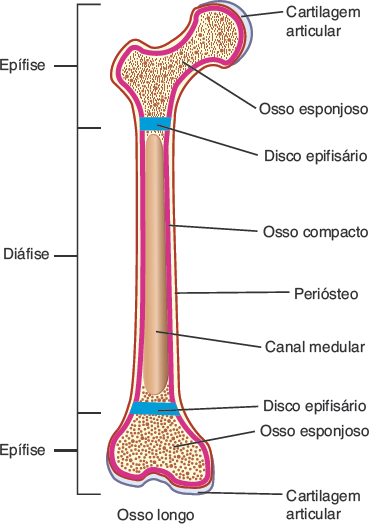
\includegraphics[width=.4\linewidth]{figures/2_theoric_foundamentations/estruturaosso.png}
        \\[\abovecaptionskip]
        \small (a)
    \end{tabular}
    \begin{tabular}{@{}c@{}}
        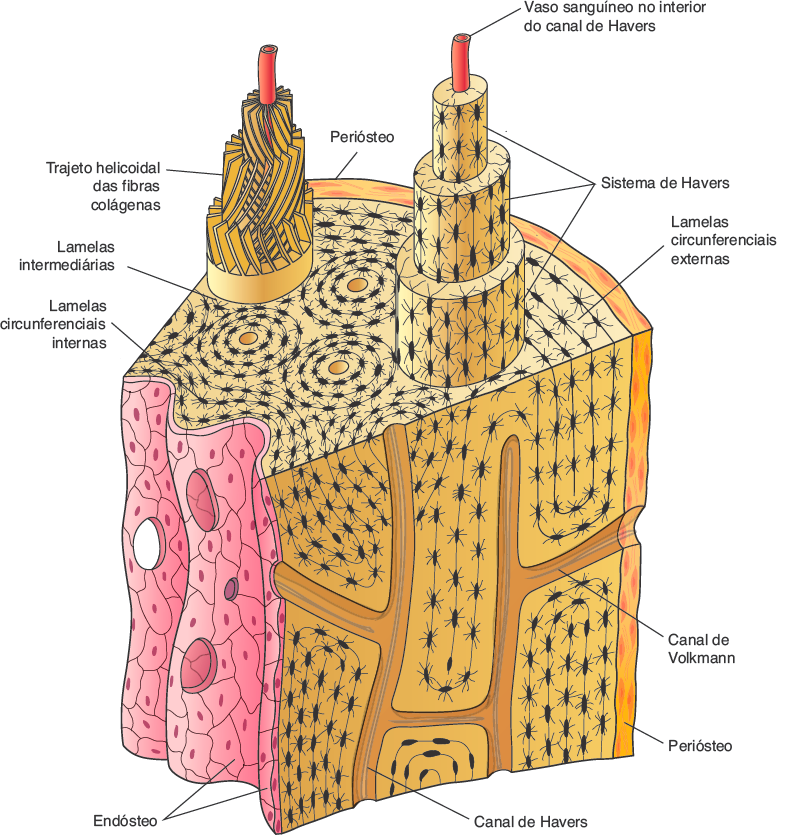
\includegraphics[width=.4\linewidth]{figures/2_theoric_foundamentations/sistemahavers.png}
        \\[\abovecaptionskip]
        \small (b)
    \end{tabular}
  
    \caption[Estrutura básica de um osso longo.]{Estrutura básica de um osso longo. Em (a) os principais componentes anatômicos de um osso longo. Em (b) os canais de Havers e Volkmann, que compõem o osso compacto, principal componente da diáfise, região intermediária de ossos longos. Fonte: \cite{junqueira1985histologia}}
    \label{fig:estrutura-ossos-longos}
\end{figure}

Os vasos sanguíneos e linfáticos que percorrem os canais nutrem os osteócitos, que são estruturas que cumprem um importante papel na manutenção e integridade da matriz óssea. Dessa forma a rede de canais ósseos cumpre um importante papel de nutrição do tecido contribuindo para seu desenvolvimento e no processo de reparo ósseo \cite{junqueira1985histologia}.

A Figura~\ref{fig:corte-canais-osteocitos} ilustra um corte transversal na diáfise de um osso longo e um exemplo de imagem histológica dessa região, destacando os canais ósseos e os osteócitos.
\begin{figure}[H]
    \centering
    \center
    \begin{tabular}{@{}c@{}}
        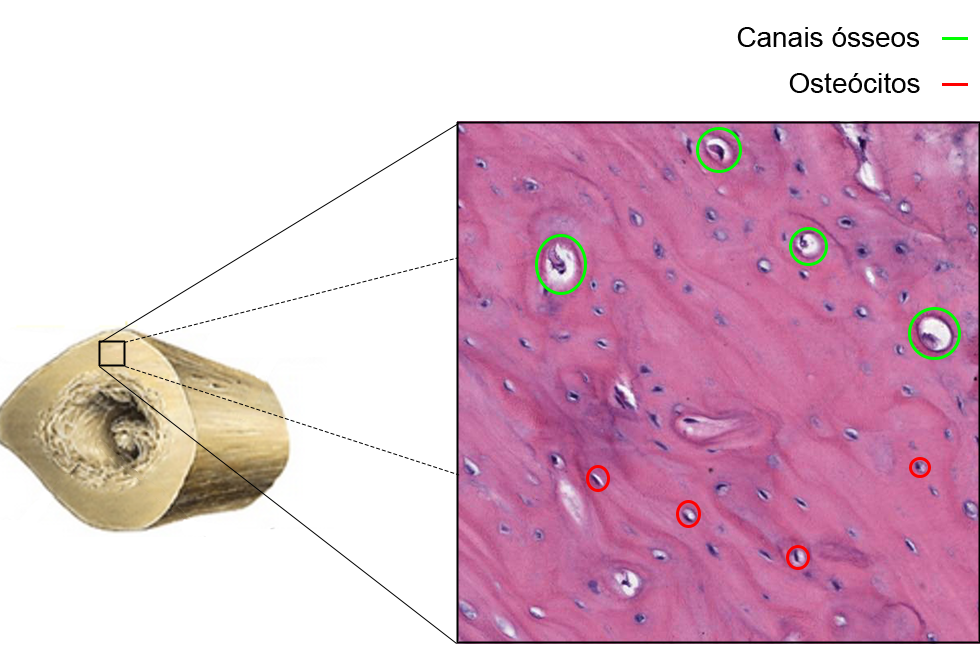
\includegraphics[width=.8\linewidth]{figures/2_theoric_foundamentations/Corte-canais-osteocitos.png}
        \\[\abovecaptionskip]
    \end{tabular}
  
    \caption[Corte transversal da diáfise de um osso longo]{Corte transversal da diáfise de um osso longo com uma região ampliada destacando alguns canais ósseos e osteócitos.}
    \label{fig:corte-canais-osteocitos}
\end{figure}

\section{Aprendizado de máquina} \label{subsec:AutoML}
Ainda em 1959 Arthur Lee Samuel definiu o aprendizado de máquina como ``o campo de estudo que dá aos computadores a habilidade de aprender sem serem explicitamente programados''~\cite{simon2013too}. De fato o aprendizado de máquinas automatizado permite, por exemplo, que computadores aprendam a realizar tarefas analisando uma base de dados previamente rotulada, além de aprimorar seu aprendizado à medida que novos dados lhe são apresentados \cite{monard2003conceitos}.

O aprendizado de máquina é um área da inteligência artificial que se apoia em técnicas e conceitos da matemática e estatística. Esse aprendizado é dividido em quatro tipos: aprendizado supervisionado, não supervisionado, auto supervisionado e por reforço. Todos possuem uma variedades de algoritmos, sendo que, para cada problema a ser resolvido, um determinado algoritmo pode ser mais adequado que os demais \cite{mueller2019deep}.

Como mencionado acima, uma das técnicas de aprendizado de máquina é o aprendizado supervisionado. Nessa abordagem utiliza-se uma base de dados na qual para cada entrada o resultado desejado é conhecido. As entradas com seus respectivos resultados esperados, também chamados de rótulos, são apresentados ao algoritmo em uma etapa conhecida como etapa de treinamento, em que o algoritmo ajusta, com base nos dados fornecidos, uma série de parâmetros internos a fim de encontrar padrões que o permitam estimar resultados para novas entradas \cite{monard2003conceitos}. A saída pode ser qualitativa, tratando-se assim de uma tarefa de classificação; ou quantitativa, tratando-se assim de uma tarefa de regressão \cite{mueller2019deep}.

\section{Aprendizado Profundo}

Uma subárea do aprendizado de máquina é o aprendizado profundo, que também trabalha com grandes conjuntos de dados para aprender a realizar tarefas. A grande diferença é que, ao invés de métodos e modelos estatísticos, o aprendizado profundo faz uso de apenas uma técnica que simula o funcionamento do cérebro humano: as redes neurais \cite{mueller2019deep}. 

Redes neurais podem possuir diversas camadas e arquiteturas, sendo que cada uma pode ser mais ou menos indicada para cada tipo de problema a ser tratado.
Tais redes são compostas por estruturas chamadas neurônios, que simulam os neurônios biológicos e se ligam uns aos outros por meio de ligações com diferentes pesos que simulam as sinapses cerebrais \cite{mueller2019deep}.

A rede neural mais simples possível é o \textit{perceptron}, que pode ser utilizada para tarefas de classificação binária ou regressão linear. O \textit{perceptron} é composto por apenas uma camada de um único neurônio. Ele recebe uma entrada $X$ de tamanho $m$ que é multiplicada por um vetor de pesos $W$ também de tamanho $m$. Em seguida é aplicada sobre o produto escalar $X \cdot W$ uma função de ativação a fim de produzir um único resultado de saída \cite{block1962perceptron}. O processo de treinamento de uma rede neural consiste justamente em realizar, com base no conjunto de dados de entrada, a parametrização do vetor de pesos $W$ das ligações entre os componentes da entrada $X$ e o neurônio \cite{mueller2019deep}.

A partir do \textit{perceptron}, novas arquiteturas de redes neurais podem ser formuladas adicionando mais camadas, mais neurônios, funções de retro-propagação de erro dentre outras estratégias que permitem que as redes neurais resolvam problemas mais complexos.

\section{Redes Neurais Convolucionais}

Desde o ano de 2012, quando a arquitetura \textit{AlexNet} venceu a competição \textit{ImageNet Large Scale Visual Recognition Challenge (ILSVRC)}, as \acf{RNC} vêm ganhando popularidade na execução de tarefas relacionadas a processamento de imagens, vídeos e até mesmo voz \cite{vargas2016estudo}.
Esse tipo de rede neural é uma variação das redes de \textit{perceptron} multicamada, e se baseia no princípio biológico da percepção visual dos seres humanos a fim de minimizar o processamento dos dados para obter o resultado esperado \cite{mueller2019deep}. São compostas por camadas convolucionais, de agrupamento, achatamento e conectada. As próximas subseções detalham o papel de cada um desses elementos.

\begin{figure}[H]
  \centering
  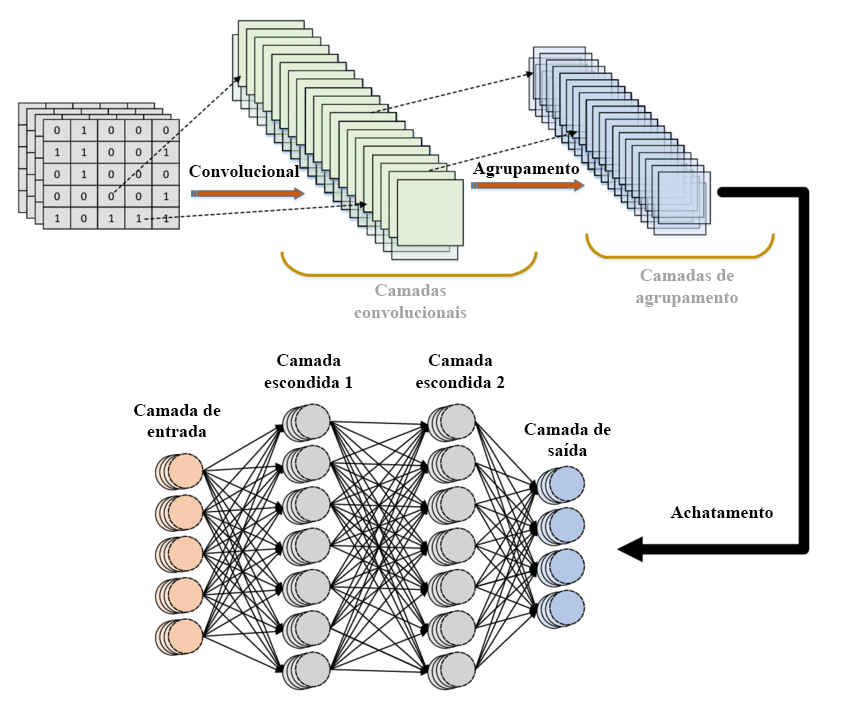
\includegraphics[width=.8\linewidth]{figures/2_theoric_foundamentations/cnn.png}
  \caption[Estrutura básica de uma rede neural convolucional.]{Exemplo de estrutura básica de uma rede neural convolucional. Imagem adaptada de \cite{srinivasan2021durld}}
  \label{fig:cnn}
\end{figure}

\subsection{Camadas convolucionais}

Na arquitetura de uma \ac{RNC}, ilustrada na Figura \ref{fig:cnn}, ao receber uma imagem como entrada são utilizadas as ditas camadas convolucionais. Tais camadas aplicam filtros (também conhecidos por \textit{kernels}), representados por matrizes tridimensionais, sobre parte da imagem de entrada \cite{rawat2017deep}.

A aplicação desses filtros se dá por um algoritmo de janela deslizante, que percorre a imagem em seus três canais de cores utilizando um passo de determinado tamanho (também conhecido como \textit{stride}) realizando uma operação de produto escalar a fim de gerar uma nova matriz cujas dimensões podem ser menores ou iguais à anterior dependendo do tamanho do filtro e do \textit{stride}. As matrizes resultantes dessa operação entre os canais de cor e os filtros são chamadas de mapas de características, e suas dimensões variam de acordo com o tamanho do filtro (\textit{kernel}) e do passo da janela deslizante (\textit{stride}). Esses são importantes parâmetros que devem ser determinados durante o projeto da rede. Esse é o processo chamado convolução, que é ilustrado pela Figura \ref{fig:conv2d} e é o mais importante processo das \ac{RNC}s \cite{geron2019maos}. 


\begin{figure}[H]
  \centering
  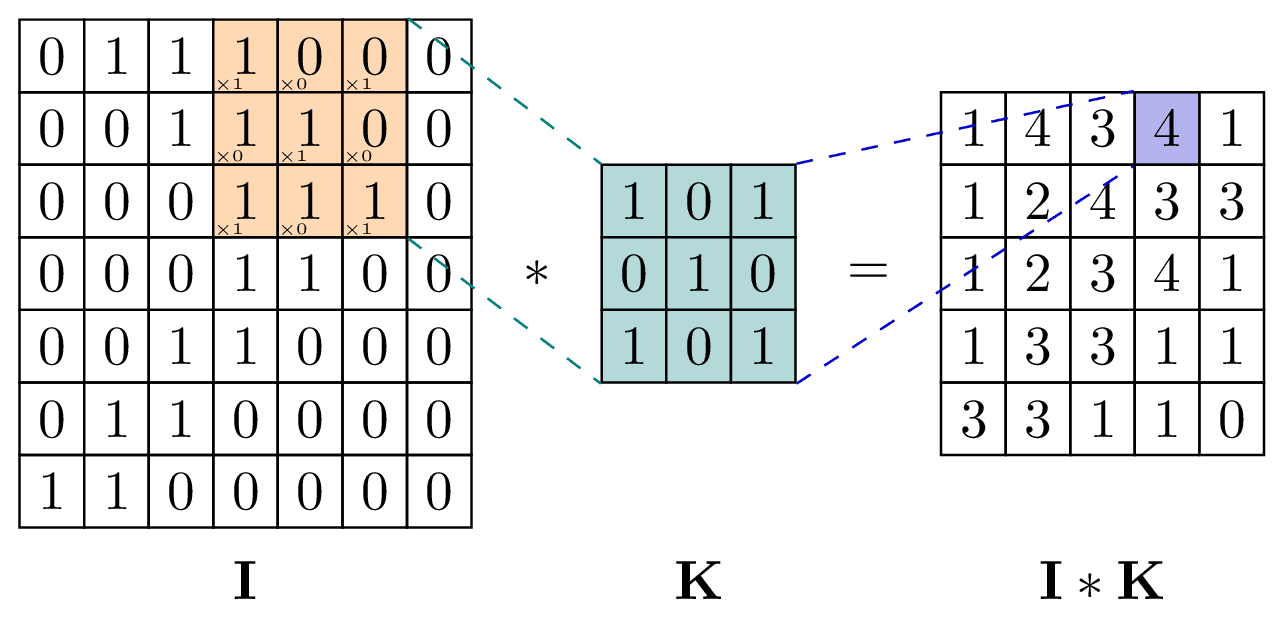
\includegraphics[width=.5\linewidth]{figures/2_theoric_foundamentations/conv2d.png}
  \caption[Exemplo de convolução entre duas matrizes bidimensionais.]{Exemplo de convolução entre duas matrizes bidimensionais. O filtro K percorre a matriz I com um passo de uma unidade calculando os produtos escalares entre a respectiva região da matriz I e o filtro K, gerando assim uma nova matriz I*K que é o mapa de características, resultado da convolução entre I e K.}
  \label{fig:conv2d}
\end{figure}

\subsection{Camadas de agrupamento}

Após cada convolução é executada outra etapa importante do processamento em \ac{RNC}s que é o agrupamento. Para esta tarefa existem as camadas de agrupamento (do inglês \textit{pooling}) cuja função é diminuir o tamanho do mapa de características visando agilidade e invariância espacial \cite{rawat2017deep}. Essa etapa consiste na utilização de uma janela deslizante a qual é aplicada uma função que seleciona um único valor para representá-la, conforme ilustrado pela Figura \ref{fig:pooling}. O uso de funções de valor máximo, mínimo e médio é bastante comum nesta etapa \cite{geron2019maos}.

\begin{figure}[H]
  \centering
  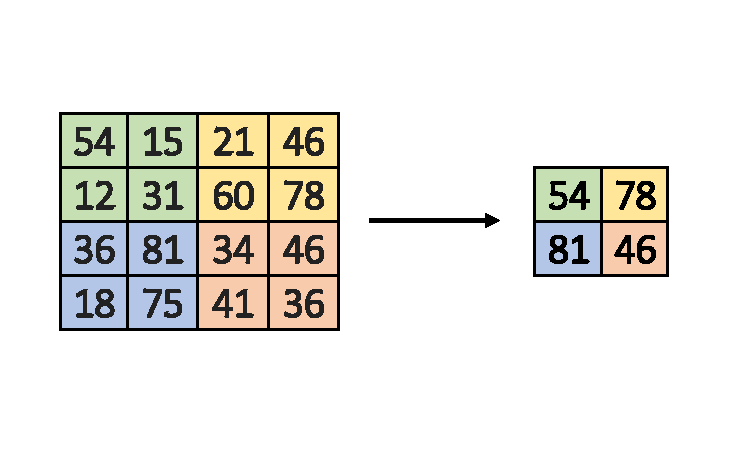
\includegraphics[width=.5\linewidth]{figures/2_theoric_foundamentations/max_pooling_example.pdf}
  \caption[Agrupamento utilizando uma função de \textit{max-pooling}.]{Exemplo de agrupamento utilizando uma função de \textit{max-pooling}. O mapa de características é percorrido por uma janela deslizante que seleciona apenas o maior valor da região para compôr um mapa de caractrísticas menor.}
  \label{fig:pooling}
\end{figure}

Devido ao fato de diminuir o tamanho da imagem de entrada, essa etapa do processo -- composta por camadas de convolução seguidas de camadas de agrupamento -- também é conhecida como caminho de contração \cite{geron2019maos}.

\subsection{Camadas de achatamento}

Após as etapas de convolução é executada uma camada de achatamento (do inglês \textit{flatten layer}), na qual os mapas de características, que são matrizes, são transformados em um vetor que será usado para alimentar uma rede de neurônios multicamada. 

\subsection{Camada densa ou conectada}
A camada que comporta a rede de neurônios é chamada camada completamente conectada (ou densa) e tem por objetivo traçar a decisão a partir dos mapas de características. Esse tipo de camada é muito utilizado em tarefas de classificação \cite{rawat2017deep}.

Uma \ac{RNC} pode apresentar outros tipos de camadas além desses tipos básicos, ou ainda não apresentar alguma das camadas mencionadas acima dependendo do objetivo da rede \cite{mueller2019deep}.

\section{U-Net}
Proposta em 2015 por \cite{ronneberger2015u}, as redes U-Net vêm sendo aplicadas em diversos trabalhos referentes à segmentação de imagens médicas, uma vez que as redes de classificação, como as \ac{RNC}s tradicionais, não conseguem trazer informações contextuais a nível de pixel, o que é essencial em tarefas de segmentação, especialmente ao se trabalhar com imagens médicas \cite{siddique2021u}. 

As redes U-Net se diferem das \ac{RNC}s de classificação principalmente devido à adição de uma etapa de decodificação. Dessa forma, após passar pelo caminho de contração o vetor de saída é novamente transformado em uma matriz e esta é ampliada por algumas camadas de aumento até chegar ao tamanho original da entrada, sendo a imagem resultante uma máscara que representa a região de interesse segmentada. Esse processo também é conhecido como caminho de expansão. A combinação do caminho de contração com o caminho de expansão resulta em uma rede quase simétrica, cujo formato lembra a letra U, conforme ilustrado pela Figura \ref{fig:u-net-example}, dando assim o nome a esse tipo de rede \cite{ronneberger2015u}.

Outra interessante característica desse tipo de rede é a ausência de uma camada conectada, sendo que esta é substituída por camadas convolucionais que processam os mapas de características com mais eficiência que uma camada conectada, conforme descrito em \cite{long2015fully}. A ausência da camada conectada, dá o nome à arquitetura das \ac{RNCC}.

\begin{figure}
  \centering
  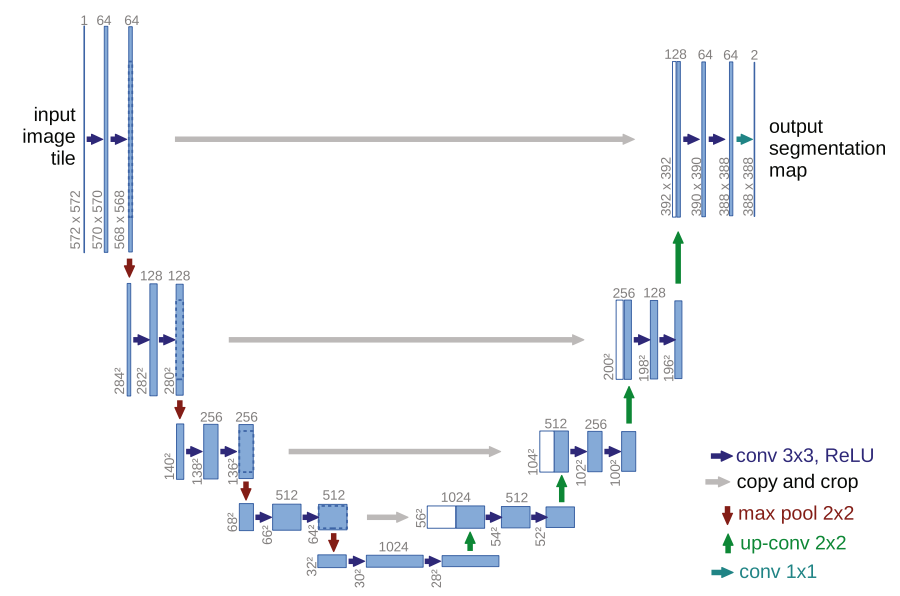
\includegraphics[width=.75\linewidth]{figures/2_theoric_foundamentations/u-net-example.png}
  \caption[Estrutura básica da rede U-Net.]{Estrutura básica da rede U-Net. Fonte: \cite{ronneberger2015u}}
  \label{fig:u-net-example}
\end{figure}

Assim, a arquitetura básica de uma U-Net, conforme foi originalmente proposta, consiste em um caminho de contração e um caminho de expansão. Durante a contração são aplicadas repetidamente duas convoluções com um filtro 3x3 seguidas de uma função de ativação \textit{ReLU} e um \textit{max-pooling} de tamanho 2x2, diminuindo em duas vezes e aumentando em duas vezes, respectivamente: o tamanho e o número dos mapas de características da saída da camada anterior \cite{siddique2021u}. 
Na expansão é feito o processo inverso: a cada camada é feito o aumento de resolução do mapa de características com uma convolução 2x2 que diminui pela metade os canais de características e dobra as dimensões da imagem (\textit{up-convolution}), uma concatenação com o mapa de características correspondente da etapa de contração e duas convoluções 3x3 seguidas por uma função de ativação \textit{ReLU}. Por fim é feita uma convolução 1x1 para mapear vetores de características para as classes desejadas. A rede possui um total de 23 convoluções \cite{ronneberger2015u}.

\section{Métricas de validação}
Esta seção apresenta e explica as principais métricas utilizadas para a validação do método proposto neste trabalho.
Para isso, consideremos a seguinte nomenclatura:

 \begin{itemize}
   \item VP - Verdadeiros positivos
   \item VN - Verdadeiros negativos
   \item FP - Falsos positivos
   \item FN - Falsos negativos
 \end{itemize}
   
\subsection{Acurácia}
A acurácia é a relação entre a quantidade de elementos classificados corretamente e a quantidade total de elementos analisados. Muitas vezes a acurácia não é a medida mais confiável para se avaliar modelos de aprendizado de máquina, pois é um desafio encontrar (e até mesmo construir) conjuntos de dados balanceados, ou seja, com aproximadamente a mesma quantidade de elementos de cada classe \cite{9075071}. Dessa forma, se um conjunto de dados para classificação binária possui um número muito mais elevado de elementos que não pertencem a uma classe C1 do que elementos que pertencem a C1, o modelo pode classificar corretamente os elementos que não pertencem a C1 e incorretamente uma boa parte dos elementos de C1 e ainda assim apresentar uma boa acurácia, visto que os elementos que não pertencem a C1 compõem a maior parte do conjunto de dados. 
A acurácia é calculada segundo a Equação \ref{eq-accuracy}.

\begin{equation}
acuracia = \frac{VP + VN}{VP + FN + FP + VN}
\label{eq-accuracy}
\end{equation}

\subsection{Especificidade}
A especificidade é a razão entre os elementos negativos que foram classificados corretamente, ou seja, os verdadeiros negativos VN; e os elementos que são de fato negativos, ou seja, a soma entre os verdadeiros negativos VN e falsos positivos FP.
Novamente, se o número de elementos negativos do conjunto de dados for muito superior ao número de elementos positivos a especificidade também pode ser uma métrica enviesada. 
A especificidade é calculada segundo a Equação \ref{eq-specificity}.

\begin{equation}
especificidade = \frac{VN}{VN + FP}
\label{eq-specificity}
\end{equation}

\subsection{Precisão}
A precisão é a razão entre o número de elementos classificados corretamente como positivos e o número de elementos que foram classificados como positivos, conforme mostra a Equação \ref{eq-precision}.

\begin{equation}
precisao = \frac{VP}{VP + FP}
\label{eq-precision}
\end{equation}

\subsection{Sensibilidade}
A sensibilidade (também conhecida como \textit{recall}) é a razão entre o número de elementos positivos classificados corretamente e o número total de elementos que são de fato positivos. A sensibilidade é calculada segundo a Equação \ref{eq-recall}.

\begin{equation}
sensibilidade = \frac{VP}{VP + FN}
\label{eq-recall}
\end{equation}

\subsection{\textit{F1-Score}}
O \textit{f1-score} (também conhecida como \textit{Dice Coefficient}) é a média harmônica entre precisão e a sensibilidade. Calculada conforme a Equação \ref{eq-dice}, busca representar a qualidade geral do modelo e é a métrica mais confiável quando se busca obter um modelo que minimize tanto os falsos positivos como os falsos negativos.

\begin{equation}
\mbox{\textit{f1-score}} = \frac{2 * precisao * sensibilidade}{precisao + sensibilidade}
\label{eq-dice}
\end{equation}

\subsection{Intersecção sobre União}
A Intersecção sobre União (\emph{Intersesction over Union -- IoU,} também conhecida como \textit{Jaccard Index}) é uma medida para calcular a similaridade entre conjuntos e é dada pela Equação \ref{eq-iou}.

\begin{equation}
\mbox{\textit{IoU}} = \frac{VP}{VP + FP + FN}
\label{eq-iou}
\end{equation}

\section{Trabalhos Relacionados}
Esta seção apresenta os principais trabalhos relacionados a esta pesquisa e que mostram técnicas de segmentação em imagens histológicas.

A literatura apresenta poucos trabalhos focados em segmentação de canais ósseos em imagens de lâmina inteira. Em \cite{liu1999bone} a segmentação foi realizada em imagens micro-radiográficas usando conhecimento em imagens ósseas e algoritmos de clusterização. As imagens de lâmina inteira se diferem das imagens micro-radiográficas especialmente em tamanho e resolução já que podem assumir ordens de giga-pixel e apresentar cores enquanto as imagens utilizadas por \cite{liu1999bone} possuíam dimensões de 512 por 576 pixels e se apresentavam em escala de cinza. A alta resolução das imagens de lâmina inteira é interessante na análise histológica devido à riqueza de detalhes que proporciona ao especialista. Porém, trabalhar com tais imagens é uma tarefa desafiadora devido ao seu tamanho, complexidade e quantidade das estruturas em relação às imagens micro-radiográficas \cite{gondim2021automatic}. 


%% Pedro
Um método para segmentação automática de canais ósseos em imagens histológicas de tecido ósseo foi proposto por \cite{gondim2021automatic}. 
Tal método processa as imagens de entrada, resumidamente, em quatro etapas: remoção de artefatos externos à matriz óssea, remoção de artefatos internos à matriz óssea, segmentação da rede vascular e remoção de falsos positivos. A cada etapa são utilizadas diversas técnicas de processamento de imagens (tais como abertura e fechamento morfológico, binarização, deconvolução de cor, etc.) em sequência e até mesmo um algoritmo de aprendizado de máquina não supervisionado denominado \textit{K-means}. Isso torna o método bastante complexo e implica em uma grande quantidade de parâmetros cujos valores devem ser fixos e obtidos empiricamente, o que leva a questionar sobre sua rebustez em relação a variações na imagem. A Figura \ref{fig:gondim-input-output} mostra um exemplo de entrada e saída do método proposto por \cite{gondim2021automatic}.

\begin{figure}[h]
    \center
    \begin{tabular}{@{}c@{}}
        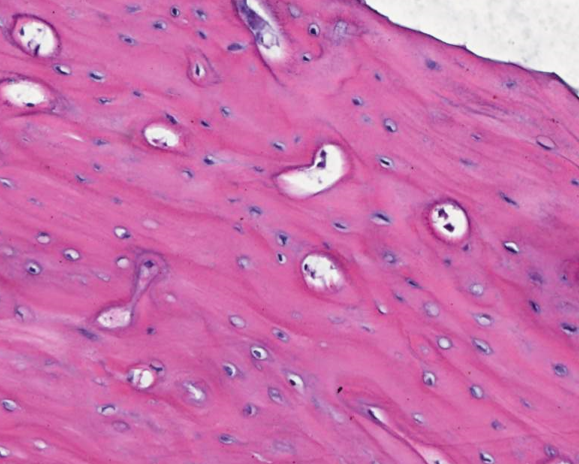
\includegraphics[width=0.3\textwidth]{figures/2_theoric_foundamentations/pedro/input.png}
        \\[\abovecaptionskip]
    \small (a)
    \end{tabular}
    \begin{tabular}{@{}c@{}}
        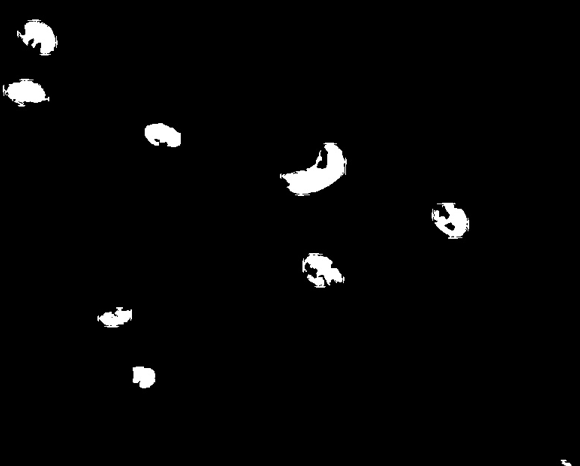
\includegraphics[width=0.3\textwidth]{figures/2_theoric_foundamentations/pedro/output.png}
        \\[\abovecaptionskip]
    \small (b)
    \end{tabular}

    
    \caption[Exemplo de entrada e saída do método proposto por \cite{gondim2021automatic}]{Exemplo de entrada e saída do método proposto por \cite{gondim2021automatic}. Em (a) imagem de entrada. Em (b) a saída do método para a entrada em (a).}
    \label{fig:gondim-input-output}
\end{figure}

Para a avaliação do método, as regiões segmentadas por \cite{gondim2021automatic} foram comparadas com marcações feitas por um especialista. 
Como as marcações manuais não seguiam a forma exata das estruturas, para comparar a segmentação do método foi considerado que se ao menos 20\% dos \textit{pixels} de uma marcação feita pelo especialista estivessem contidos na região segmentada pelo método, então a estrutura foi corretamente segmentada. Isso deixa uma lacuna em relação à forma da região segmentada pois tais formas não puderam ser validadas devido às marcações manuais, pois estas foram feitas colocando um círculo envolvendo cada canal, como mostra a Figura \ref{fig:gondim-bad-labelling}.

\begin{figure}[H]
  \centering
  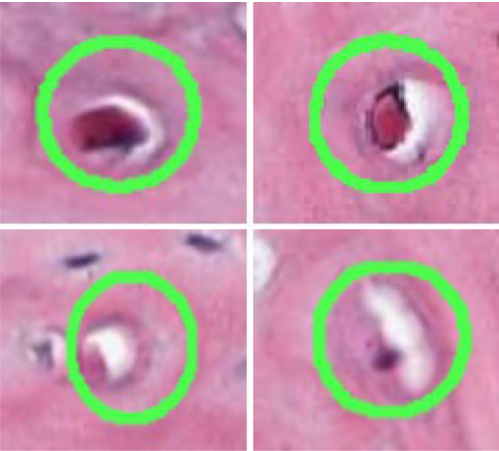
\includegraphics[width=.3\linewidth]{figures/2_theoric_foundamentations/pedro/bad_labelling.png}
  \caption[Exemplo de marcações feitas pelo especialista em \cite{gondim2021automatic}]{Exemplo de marcações feitas pelo especialista. Fonte \cite{gondim2021automatic}.}
  \label{fig:gondim-bad-labelling}
\end{figure}



%% Julia
Outra abordagem foi testada por \cite{julia2021histological}, que, na intenção de segmentar canais ósseos em imagens histológicas geradas a partir do fêmur de ratos, modificou uma rede neural convolucional do tipo \textit{U-Net} que originalmente havia sido feita para segmentação de anormalidades FLAIR em imagens de ressonância magnética cerebral. Entretanto os resultados da marcação automática feita pela \ac{RNC} implementada não foram satisfatórios devido à falta de precisão das marcações manuais feitas nas imagens, o que é ilustrado pela Figura \ref{fig:julia-results}. O modelo treinado apresentou sobreajuste e alcançou um \textit{Dice Coefficient} de apenas 20\%.

\begin{figure}[h]
    \center
    \begin{tabular}{@{}c@{}}
        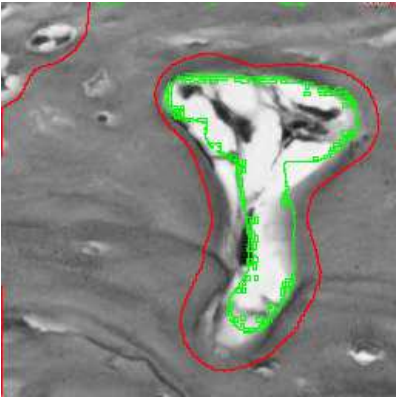
\includegraphics[width=0.3\textwidth]{figures/2_theoric_foundamentations/julia/result1.png}
    \end{tabular}
    \begin{tabular}{@{}c@{}}
        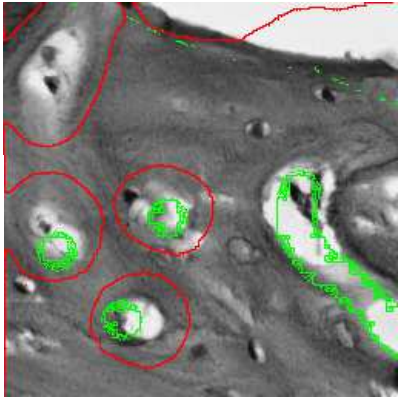
\includegraphics[width=0.3\textwidth]{figures/2_theoric_foundamentations/julia/result2.png}
    \end{tabular}

    
    \caption[Exemplos de saídas do método proposto em \cite{julia2021histological}.]{Exemplos de saídas do método proposto. Em verde a saída da rede neural, em vermelho a marcação provida pelo especialista. Imagem adaptada de \cite{julia2021histological}.}
    \label{fig:julia-results}
\end{figure}

Como proposta de melhoria em seu trabalho, \cite{julia2021histological} sugere o uso de um conjunto de imagens com marcações mais precisas, a fim de melhorar os resultados da \ac{RNC}.

Em ambos os trabalhos observa-se que a qualidade do conjunto de imagens teve impacto negativo na avaliação dos resultados da segmentação. Acredita-se que um conjunto de imagens com marcações mais precisas e confiáveis em relação ao tamanho, forma e posição das estruturas de interesse pode levar a um resultado mais preciso, e o uso de redes neurais convolucionais pode resultar em um método mais robusto quanto à invariância, apresentando assim mais flexibilidade ao tratar imagens com características diferentes. 



%% DALI
Pensando nos bons resultados que as redes neurais convolucionais têm apresentado no processamento de imagens nos últimos anos, \cite{Santos2021} utiliza redes neurais convolucionais para segmentar regiões tumorais em imagens de lâmina inteira de tecido oral, obtendo bons resultados, como cerca de 97.6\% de acurácia, 98.4\% de especificidade e 92.9\% de sensibilidade. Foi utilizada uma \ac{RNCC} baseada no modelo \textit{U-Net} treinada com uma base de imagens, desenvolvida pelos autores, que continha imagens histológicas de tecidos da cavidade oral corados com \ac{HE}.

Antes do treinamento foi feita uma etapa de pré-processamento para identificar as regiões de tecido, descartando áreas desinteressantes para o trabalho.
As imagens eram então divididas em sub-imagens e apresentadas à rede para o treinamento, que também contava com uma estratégia de aumento de dados. 
O resultado da rede era uma imagem em escala de cinza em que era calculada para cada pixel da imagem a probabilidade $p$ de tal pixel pertencer ou não à região de interesse. Por fim eram marcados como positivos os pixels que apresentassem $p$ acima de um \textit{threshold} de 50\%, valor este que foi escolhido empiricamente. A Figura \ref{fig:dali-results} apresenta exemplos dos principais elementos gráficos presentes no método proposto por \cite{santos2022automated}.

\begin{figure}[h]
    \center
    
    \begin{tabular}{@{}c@{}}
        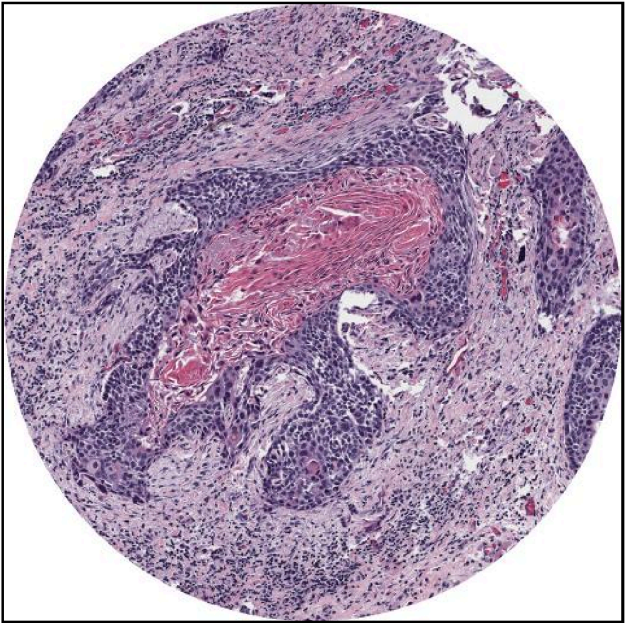
\includegraphics[width=0.18\textwidth]{figures/2_theoric_foundamentations/dali/input.png}
        \\[\abovecaptionskip]
    \small (a)
    \end{tabular}
    \begin{tabular}{@{}c@{}}
        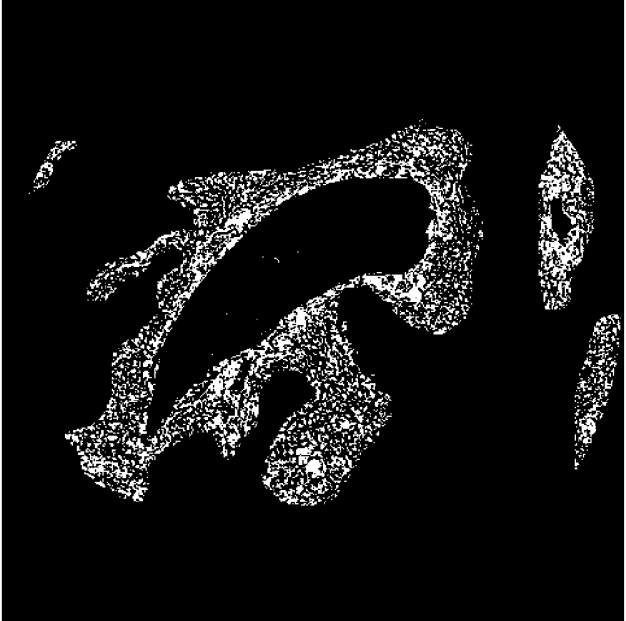
\includegraphics[width=0.18\textwidth]{figures/2_theoric_foundamentations/dali/gold_standard.png}
        \\[\abovecaptionskip]
    \small (b)
    \end{tabular}
    \begin{tabular}{@{}c@{}}
        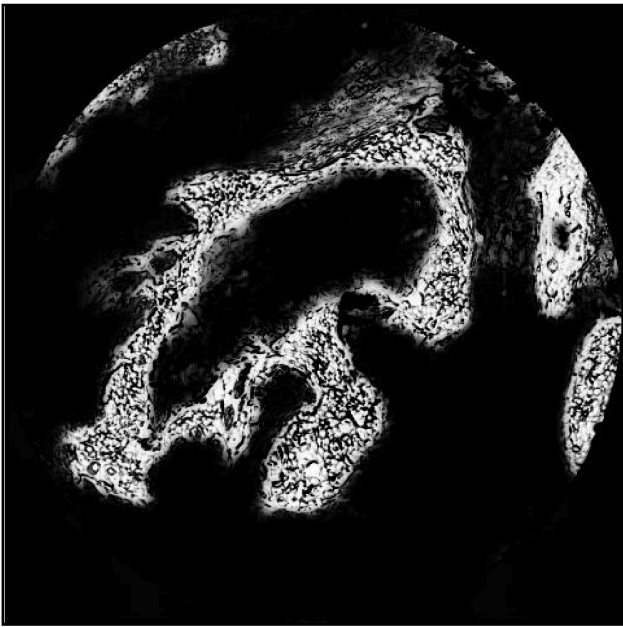
\includegraphics[width=0.18\textwidth]{figures/2_theoric_foundamentations/dali/probabilidades.png}
        \\[\abovecaptionskip]
    \small (c)
    \end{tabular}
    \begin{tabular}{@{}c@{}}
        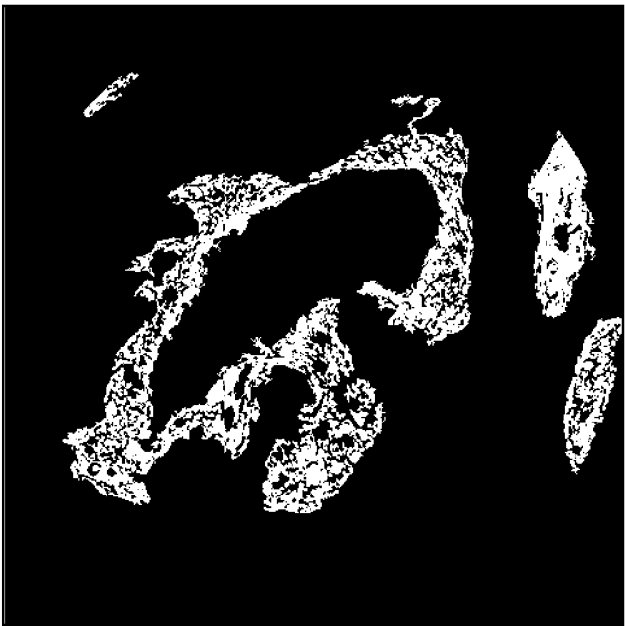
\includegraphics[width=0.18\textwidth]{figures/2_theoric_foundamentations/dali/net_output.png}
        \\[\abovecaptionskip]
    \small (d)
    \end{tabular}
    \begin{tabular}{@{}c@{}}
        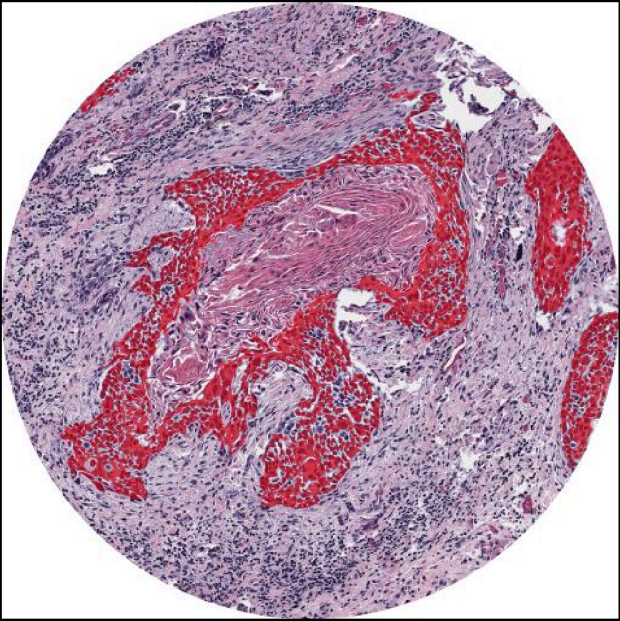
\includegraphics[width=0.18\textwidth]{figures/2_theoric_foundamentations/dali/final.png}
        \\[\abovecaptionskip]
    \small (e)
    \end{tabular}

    
    \caption[Principais elementos gráficos presentes no método proposto por \cite{santos2022automated}.]{Exemplos dos principais elementos gráficos presentes no método proposto por \cite{santos2022automated}. Em (a) uma imagem de entrada. Em (b) um exemplo de marcação padrão ouro. Em (c) um exemplo da saída da rede, em que cada pixel é preenchido de acordo com a probabilidade de pertencer à região de interesse (quanto mais próximo da cor branca, maior a probabilidade). Em (d) a marcação final do método, com \textit{threshold} de 50\%. Em (e) a região com tumor representada em vermelho na imagem original. Imagem adaptada de \cite{santos2022automated}.}
    \label{fig:dali-results}
\end{figure}

O método também foi validado em outras bases de imagens presentes na literatura, e apresentou um \textit{f1-score} de 90\% na base desenvolvida pelos autores e média geral de 83\%. Além disso o método foi testado com diferentes tamanhos de sub-imagens -- o melhor resultado foi obtido para sub-imagens de tamanho 640x640 pixels.
